% RQ1
\section{Empirical study}
\label{sec:empiricalstudy}
% Both state of the art tools
% But also commonly used simpler tools
To substantiate further research questions with research data, a empirical study on error detection tools and different configurations is designed. To cover a broad range of configurations (strategies) of these tools, a range of permutations of configurations will be generated for each error detection tool and run on a wide range of datasets with different characteristics and errors. The source code of this framework can be found on GitHub\footnote{\url{\githubsource}}.
~\\Because the source languages of error detection tools differ, a high-level general purpose programming language suits to be used for the framework to connect all the different underlying tools. Together with the fact that it has well-supported libraries for relational data handling, Python\footnote{\url{\pythonsource}} was chosen as the main development language.


\subsection{Setup}
\label{subsec:setup}
First, the setup for the empirical study will be discussed. The basic setup is shown in figure \ref{fig:empiricalsetup}. For each tool in the study, a number of configurations is created, depending on the configurability of the tool. Each configuration in combination with that tool, will be tested on all the available datasets. So a single experiment exists of:
\begin{itemize}
    \item An error detection tool
    \item A tool specific configuration
    \item A target dataset
\end{itemize}

Each experiment will be pushed to the queue of experiments, allowing for retrieving a experiment session without having to rerun all the finished experiments. Incrementally, all the experiment results are pushed into the results database, allowing for the empirical study and further usage with performance prediction and tool ranking. 

\begin{figure}[h]
    \centering
    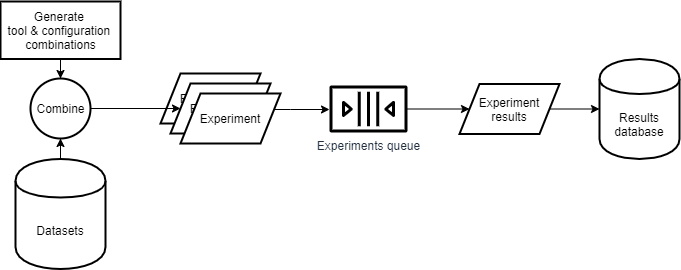
\includegraphics[width=\textwidth]{thesis/Figures/EmpiricalStudy.png}
    \caption{Setup of the empirical study}
    \label{fig:empiricalsetup}
\end{figure}

% Error detection API to do experiments
\subsection{Error detection framework}
First, a framework for running error detection tools was designed. The purpose of creating a single framework is to have homogeneous in and output for each selected error detection strategies, creating the possibility of running batches of experiments in a structured manner. 
The structure of the error detection framework is as follows:
\begin{

\subsection{Metrics}
\label{subsec:metrics}
To measure the performance of tools on test datasets, metrics of two types can be used. Cell-based and row-based metrics. The difference lies in what is taken as an entity while calculating scores.

\subsubsection{Cell-based metrics}
Cell-based metrics, are metrics that identify each cell in a dataset as a separate entity in the test set. Each cell will be counted as 1 positive or negative. 

\subsubsection{Row-based metrics}
Row-based metrics, are metrics that identify each row in a dataset as a separate entity in the test set. A row could contain multiple errors, but only the whole row is counted as 1 positive or negative.
\todo{Add visual example of scores \& row vs. cell based metrics}

\subsubsection{Scores}
In the case of error detection, instances are either erroneous (positive) or clean (negative). Because the ground truth of the datasets in section \ref{subsec:datasets} is known, the following metrics can be calculated directly after the execution of a tool.

\paragraph{Accuracy}
is the metric consisting of the sum of all true positives and true negatives, divided by the total number of instances. Whenever working with imbalanced datasets, this number could give a misleading confidence in the score, whereas the larger type (positives or negatives) dominates the score.

\paragraph{Precision}
is the metric consisting of the count of all true positives, divided by all the true positives and false positives. This metric is the fraction of relevant instances among all the "detected" positives. High precision means that the quality of errors detected is good, without having a large fraction of false positives. This metric could be helpful for completely automated processes. If precision is 1, no mistakes were made in the detected errors and no human interaction is needed. This metric however does not tell anything about the portion of total errors retrieved and errors still left in the dataset, only about the quality of the instances predicted to be errors.

\paragraph{Recall} 
is the metric consisting of the count of all true positives, divided by the count of all true positives and false negatives. Whereas precision measures the quality of positively labeled instances, recall is the fraction of correctly detected errors divided by the total number of true errors in the dataset. This metric focuses on retrieving all errors from the dataset, without any regard for the quality of the predictions.

\paragraph{F1-score}
is the metric that is the harmonic mean of precision and recall. So it is a combination of both recall and precision, measuring each score with equal importance. Due to this mix of importance, it is usable as a single metric, while having a larger scope of measurement.
~\\The F1-score (also F-measure), will be the main goal to estimate in later sections.

\subsection{Datasets}
\label{subsec:datasets}
The datasets selected contained different types of errors, to create a heterogeneous test set to compare the tools and configurations. Errors in a dataset are defined by the difference in the dirty dataset and clean dataset. So only the ground truth makes up an error. Errors can be seen as a transformation of the ground truth to some dirty value. These transformations could specify why the dirty version is wrong. Below are different "error types" that describe errors that have similar transformation between the dirty instance and the ground truth. Of course, there might be overlap in these transformation, as one type of transformation could have the same effect as another type, but these categorizations give an overview of the dataset quality one has to deal with.

\subsubsection{Error types}
\begin{itemize}
    \item \textit{Wrong patterns:} Values that are erroneous and do not fit in the common pattern of that column (i.e. 2k20 in stead of 2020)
    \item \textit{Missing values:} Empty values or missing value placeholders (N/A) that are replaced are supposed to be a real value
    \item \textit{Wrong content:} An error value where the content of the entity is changed, i.e. wrong categories, description or other matters that change the meaning of the underlying value.
    \item \textit{Spelling errors:} Error values where content and pattern is correct, but with wrong spelling.
    \item \textit{Inconsistent representations of entities:} Inconsistent abbreviations or references to entities (like states, companies, universities, etc..)
    \item \textit{Numerical outliers:} Numerical values that are erroneous and do not fit in the (column) distribution of the dataset
    \item \textit{Classification errors:} Values that are result of a classification (output) based on the other given columns, but the output is wrong
\end{itemize}

(1 ED2 \cite{Neutatz2019-aw}, 2 Raha \cite{Mahdavi2019-zf}, 3 CleanML \cite{Li2019-ve}, 4 REDS \cite{Mahdavi2019-pk})
\todo{Paragraph for each dataset used}

A summary of the list of datasets used for the empirical study, performance estimation and ranking of error detection strategies can be found below (table \ref{tab:datasets}).
~\\
\begin{table}[H]
\begin{adjustbox}{tabular=lllll,center}
Name        & Error types \\ \hline
Beers & Wrong patterns \& missing values                              \\
Flights                          & Wrong patterns \& missing values                              \\
Hospital   & Spelling mistakes \& wrong patterns                        \\
Rayyan                           & Wrong patterns, wrong content \& missing values              \\
Tax                                       & Wrong patterns                                            \\
Toy                           & Missing values \& wrong content                           \\
Restaurants          & Wrong patterns, wrong content \& missing values                  \\
Restaurant    & Pattern errors \& spelling errors                         \\
Movies               & Pattern errors, wrong content \& missing values               \\
Movie             & Inconsistent representations of entities                  \\
University                       & Inconsistent representations of entities                     \\
Uscensus                                  & Missing values, wrong content \& classification errors    \\
KDD          & Wrong content, numerical outliers \& classification errors   \\
EEG                              & Numerical outliers \& classification errors                  \\
Company     & Wrong patterns                                                        \end{adjustbox}
\caption{Table with different datasets used, a small description, the common error types and their source}
\label{tab:datasets}
\end{table}

\subsection{Tools}
\label{subsec:tools}
In this subsection, the tools used in the case study will be discussed. The extensive summary of the workings of the tools can be found in section \ref{chap:background}.

\subsubsection{Raha \cite{Mahdavi2019-zf}}
A human-guided but configuration-free error detection system. It selects different preconfigured strategies automatically, based on previously cleaned datasets. Then, it incorporates the \textbf{outputs from various error detection strategies} as a feature vector for the error detection task. Using these feature vectors, it creates clusters of which samples will be labeled in order to reduce user involvement.

\subsubsection{Forbidden Itemsets \cite{Rammelaere2019-ea}}
Applies \textbf{constraint-like method} to detect and repair invalid entries in a dataset. The proposed so-called forbidden itemsets capture unlikely value co-occurrences, similar to denial constraints.

\subsubsection{FAHES \cite{Qahtan2018-te}}
A disguised missing values detector. Whereas most missing value detector focus only on NULL or empty values, this tool takes a different approach. They \textbf{categorize detectable disguised missing values} into five different cases: 1. Out of range data values 2. Outliers 3. String with repeated characters or characters that are next to each other on the used keyboard 4. Values with non-conforming data types 5. Valid values that are randomly distributed within the range of the data and used frequently in the data set.

\subsubsection{HoloClean \cite{Rekatsinas2017-iw}}
HoloClean, a data cleaning system that relies on \textbf{statistical learning and inference} to unify a range of data repairing methods. Contributions in this tool include: 1. a compiler that generates a probabilistic model which unifies different signals for repairing a dataset 2. an algorithm that uses Bayesian analysis to prune the domain of the random variables corresponding to noisy cells in the input dataset to systematically tradeoff the scalability and quality of repairs 3. an approximation scheme that relaxes hard integrity constraints to priors over independent random variables.

\subsubsection{dBoost \cite{Pit--Claudel2016-dj}}
Outlier Detection in Heterogeneous Datasets using Automatic Tuple Expansion. It uses \textbf{expansion of data tuples using knowledge about the schema and field types}. For example, a timestamp 1424866716 could be expanded into year 2015, Wednesday, etc.. Then outliers are detected based upon these schemas.

\subsubsection{KATARA \cite{Chu2015-fs}}
A \textbf{knowledge base} and crowd powered data cleaning system that, given a table, a knowledge base, and a crowd, interprets table semantics to align it with the knowledge base. Identifies correct and incorrect data, and generates top-k possible repairs for incorrect data.

\subsubsection{ActiveClean \cite{Krishnan2016-rg}}

\subsubsection{Adapted tools}
\label{subsubsec:adaptedtools}
